\documentclass[12pt]{article} % Aqui defines que tipo de documento es, el tamaño de letra y otros detalles. ignora las advertencias y errores, peo mantente al tanto de que si no compila el documento por que usualmente aparecen aqui las advertencias y soluciones.
\usepackage[spanish]{babel} % Este paquete es para que el formatos como la fecha o secciones como abstract esten en español
\usepackage{csquotes} % Este paquete es para que las citas en el texto esten en español
\usepackage{multicol} % Este paquete es para simplificar el uso de columnas
\usepackage{fullpage} % Este paquete es para que el documento ocupe toda la pantalla
\usepackage{amsmath} % Este paquete añade ambientes para alinear ecuaciones y otros detalles matematicos
\usepackage{graphicx} % Este paquete es para incluir imagenes
\usepackage{listings} % Este paquete es para incluir códigos
\usepackage{xcolor} % Este paquete es para definir colores
\usepackage{tabularx} % Este paquete es para definir tablas con un ancho especifico
\usepackage{hyperref} % Este paquete es para incluir hipervinculos
\usepackage[export]{adjustbox} % Este paquete es para ajustar imagenes, mas especificamente para quitar un par de errores
\usepackage{float} % Este paquete es para resolver los problemas de los abientes figure cuanto estan en 2 columnas
\usepackage[backend=biber]{biblatex} % Este paquete es para incluir bibliografias
\lstdefinestyle{mystyle}{ % Aqui estoy definiendo los colores y estilos para los codigos
    backgroundcolor=\color{black!5},
    commentstyle=\color{green!60!black},
    keywordstyle=\color{blue},
    numberstyle=\tiny\color{gray},
    stringstyle=\color{purple},
    basicstyle=\footnotesize\ttfamily,
    breakatwhitespace=false,
    breaklines=true,
    captionpos=b,
    keepspaces=true,
    numbers=left,
    numbersep=5pt,
    showspaces=false,
    showstringspaces=false,
    showtabs=false,
    tabsize=2
}
\lstset{style=mystyle} % Aqui estoy aplicando el estilo definido arriba

\addbibresource{refs.bib} % Aqui se define el archivo .bib con las referencias
\bibliography{refs.bib} % Aqui se define que la bibliografia es ese archivo. La neta no se por que pero si no lo pongo no funciona

\begin{document} % Empezamos el documento
\vspace*{-3cm} % Los comandos vspace* y hspace* son para mover cosas en el documento, en este caso estoy moviendo las imagenes y el titulo un poco mas arriba
\begin{center} %Logos
    \begin{minipage}[t]{0.3\textwidth} % El ambiente minipage ayuda a ubicar figuras e imagenes en el documento cuando se tienen multiples columnas
        \centering
        
\includegraphics[width=1\textwidth]{Logos/UASLP.png} 
    \end{minipage}
    \hfill
    \begin{minipage}[t]{0.3\textwidth}
        \centering
        
\includegraphics[width=0.8\textwidth]{Logos/FCIENCIAS.png}
    \end{minipage}
    \hfill
    \begin{minipage}[t]{0.3\textwidth}
        \centering
        
\includegraphics[width=0.8\textwidth]{Logos/IICO.png}
    \end{minipage}
    \hfill
\end{center}
\vspace*{0.5cm}
\begin{center} % El ambiente center es para centrar cosas, en este caso el titulo, fecha, nombres, etc
{\LARGE \textbf{Plantilla de Reportes IICO}} \\[0.3cm] %Aqui va el titulo del reporte
{\Large Un tutorial de \LaTeX} \\[0.2cm] %Aqui va el nombre del curso y El profesor, o lo que quieras poner de subtitulo
{\large \today} \\[0.2cm] %Fecha una opcion es poner la fecha de entrega
{\large Leonides Jonguitud-Rodriguez} %nombres de los integrantes del equipo
\end{center}
\vspace*{-8mm}
\begin{abstract}
\vspace*{-5mm}
\hspace{-2cm} % Aqui hago varios ajustes para añadir lineas horizontales antes y despues del abstract
\noindent\rule{17cm}{0.4pt}\\ % Aqui ya pones tu abstract
Este documento, tanto su formato de salida como su código fuente, es un tutorial de como utilizar \LaTeX para escribir un reporte de laboratorio. El texto aquí mostrado delineara el proceso de investigación, diseño, y experimentación que a mi como autor me ha funcionado mientras expone un pequeño tutorial de la instalación simplificada para programar \LaTeX en una maquina Windows. Al final de la lectura y análisis de este documento y sus archivos adjuntos, principalmente el archivo fuente adjunto (.tex), se espera que el lector tenga una comprensión básica tanto del método de escritura e investigación preferido por el autor, como una capacidad de programar y utilizar las librerías principales de \LaTeX para escribir un documento propio, o en su defecto utilizar esta plantilla a su máximo potencial.\\
\hspace*{-40pt}
\rule{17cm}{0.4pt}
\end{abstract}

\begin{multicols}{2} % Aqui comenzamos el ambiente de dos columnas para el contenido principal del documento
\section{Introduccion} 

\section{Simulación}

\section{Conclusiones}
\begin{figure}[H] % Aunque sea posible solamente añadir imagenes directamente con el comando includegraphics, es recomendable usar el ambiente figure para añadir leyendas y referencias cruzadas. El [H] es para forzar a que la imagen se quede en el lugar donde esta en el codigo
    \centering % centramos la figura
    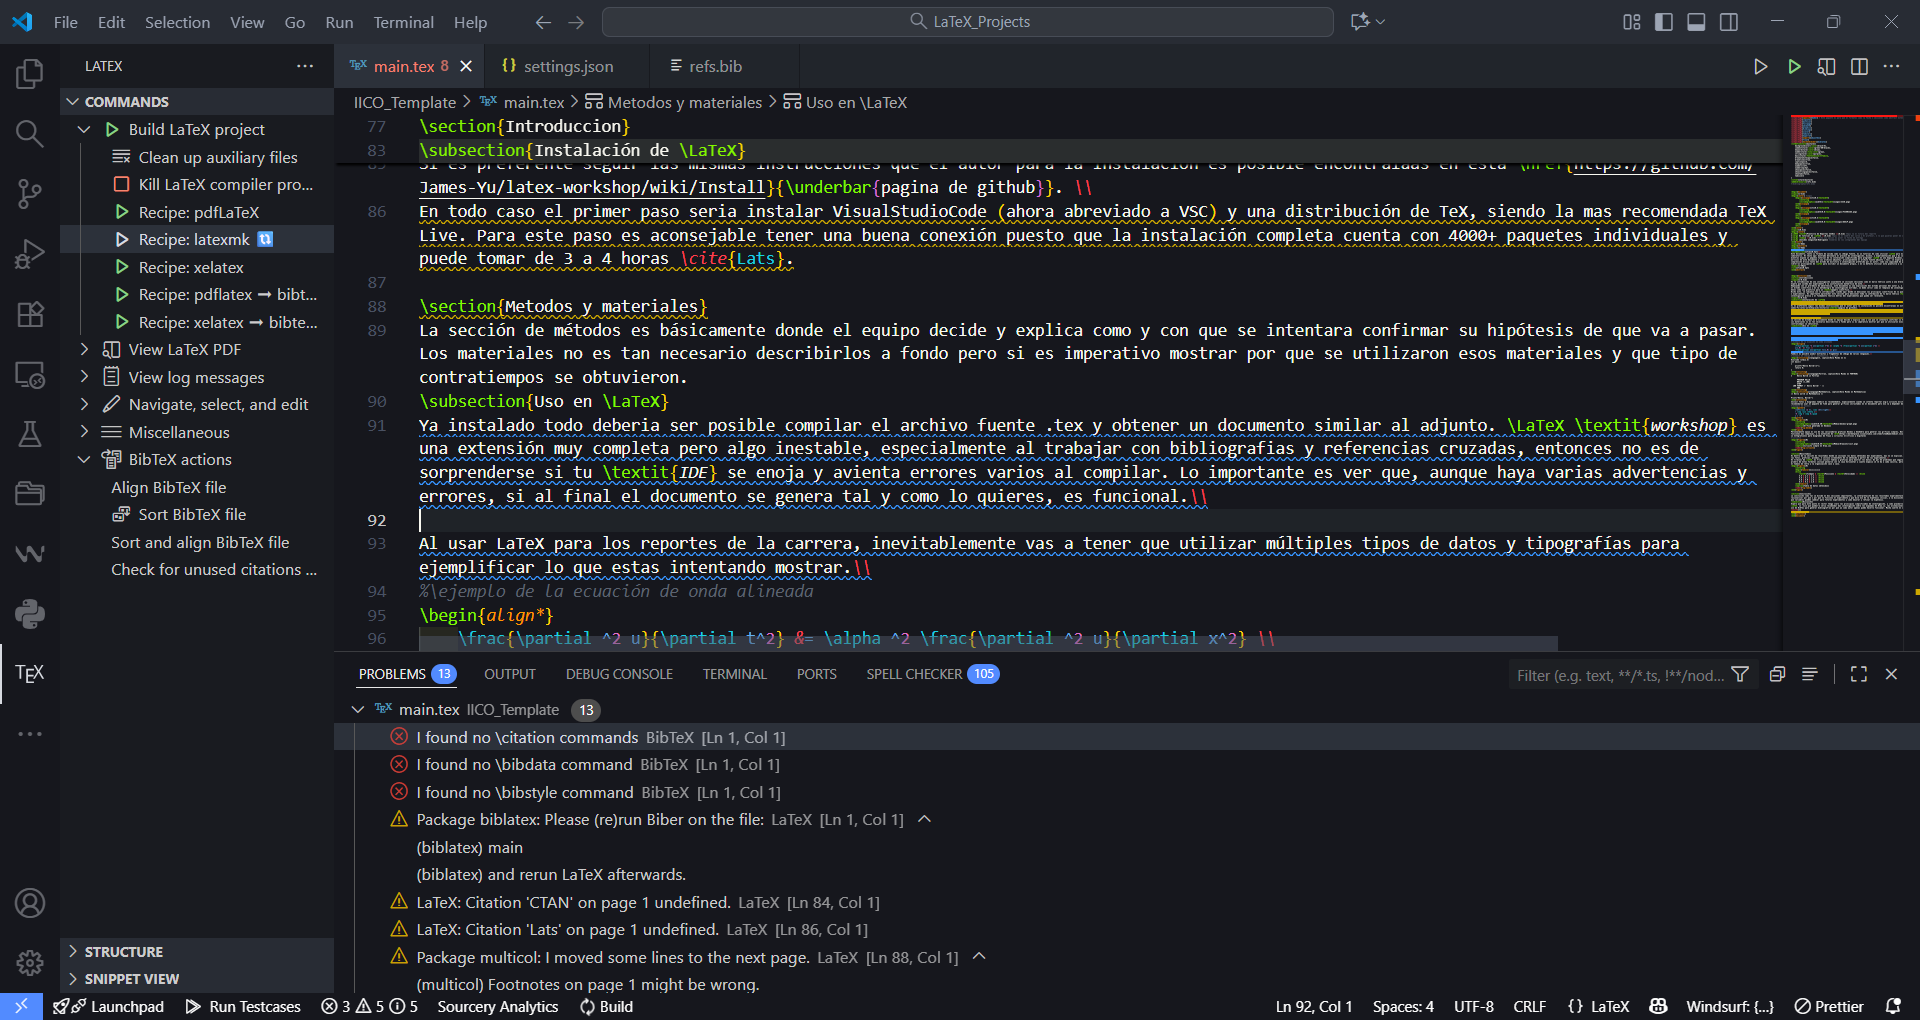
\includegraphics[width=0.45\textwidth]{Media/VSC_Screenshot-errors.png} % El comando includegraphics es para incluir imagenes, el parametro width es para definir el ancho de la imagen en proporcion al ancho del texto
    \caption{Visual Studio Code con LaTeX Workshop, notese los errores en la consola.} % El comando caption es para añadir una leyenda a la imagen
    \label{fig:vscode} % El comando label es para definir una etiqueta para referencias cruzadas en el texto fuera de la figura
\end{figure}
% Para ecuaciones y expresiones matemáticas, el paquete AMSMath es el mas completo y recomendable. El ambiente equation es para ecuaciones numeradas y centradas en la columna, mientras que align es para ecuaciones alineadas por un símbolo en particular (&), usualmente el signo igual.\\
\begin{align*}
    \frac{\partial ^2 u}{\partial t^2} &= \alpha ^2 \frac{\partial ^2 u}{\partial x^2} \\
    u(x,0)  &= f(x) \\
    \frac{\partial u}{\partial t}(x,0) &= g(x)
\end{align*}
\begin{lstlisting}[language=C, caption=Hola Mundo en C]
#include <stdio.h>
int main()
{
    printf("Hello World!\n");
    return 0;
}
\end{lstlisting}

Incluir fotos y diagramas también es recomendable, especialmente cuando se intenta reportar algún circuito eléctrico. Muchas fuentes recomendaran usar el paquete de TikZ para generar gráficos incrustados en el documento pero eso va a depender de que aplicación se use.
% No uses TikZ para circuitos, usa Draw.io, no vale la pena

\begin{gather} % El ambiente gather es para incluir ecuaciones centradas en la columna pero sin alineacion o nuemracion
    \left(\sin (2 t), \cos (3t)\right)\\
    r \leq \sin \theta s\\
    -5 \leq t \leq 5;\quad
    s = -7
\end{gather}
\begin{figure}[H] % Aunque sea posible solamente añadir tablas directamente con el comando tabular, es recomendable usar el ambiente figure para añadir leyendas y referencias cruzadas. El [H] es para forzar a que la tabla se quede en el lugar donde esta en el codigo
    \centering
    \begin{tabular}{|c||c|c|} % Al definir la tabla, las letras entre llaves definen el numero de columnas y su alineacion (c=centrado, l=izquierda, r=derecha), las lineas verticales | son para definir lineas verticales en la tabla. A cada paso se le agrega un \hline
    \hline
        \textbf{Tiempo} & \textbf{Posicion} & \textbf{Velocidad} \\ \hline
        3.4 & 2.2 & 1.2 \\ \hline
        4.5 & 3.1 & 1.4 \\ \hline
        5.6 & 4.0 & 1.6 \\ \hline
        6.7 & 5.2 & 1.8 \\ \hline    
    \end{tabular}
    \caption{Tabla de datos obtenidos}
    \label{fig:tabla}
\end{figure}
\nocite{*} % El comando nocite{*} es para que se muestren todas las referencias del archivo .bib aunque no hayan sido citadas en el texto
\printbibliography % El comando printbibliography es para imprimir la bibliografia en el documento
\end{multicols}
\end{document}